% File: SpringBlocks.tex
% Author: Adam Leeper
%------------------------------------------------------------------------------
\providecommand{\isolatedBuild}[1]{#1}% Fallback definition to build normally.
\isolatedBuild{
  \documentclass[11pt,letterpaper]{book}
  %\documentclass[11pt,letterpaper]{book}

% aleeper: I think these are needed for Paul's macros?
\usepackage{epsfig}
\usepackage{epstopdf}

%\makeatletter
%\typeout{The import path is \import@path}
%\makeatother

\usepackage{import}

\subimport{./}{packagesMitiguy.sty}
\subimport{./}{macrosMitiguy.tex}
\subimport{./}{PageStylesMitiguy.tex}
\subimport{./}{macrosLeeper.tex}
   % Found via TEXINPUTS environment variable.
  \isolatedBuildHeader{Newton's Law for a Translating System}
                      {Dynamics of a Mass-Spring System with a Jet Engine}
}
%%%
%%%
%%%
Blocks \basis{A} (with mass $m^A = 1$ kg) and \basis{B}
(with mass $m^B = 2$ kg), modeled as particles, slide on a smooth surface
\basis{N} (taken to be a Newtonian reference frame). Gravity acts ``downward."
A spring of stiffness $k = 200$ N/m and natural length $L_N = 1$ m connects
the blocks. Additionally, block \basis{A} has a jet thruster on it which
produces a force $(F_x~\uvecx{n})$ on \basis{A}.
The variable $x_A$ is the \uvecx{n} measure of the distance from $N_o$ to A,
and the variable $x_B$ is the \uvecx{n} measure of the distance from \basis{A}
to \basis{B}.

\begin{center}
  \includegraphics[width=0.45\linewidth]{spring_blocks.png}
\end{center}

\begin{enumerate}
\item Find expressions for the acceleration of each block in \basis{N}.
\item Form \force{A}, the resultant force on \basis{A}, and \force{B},
  the resultant force on \basis{B}.
\item When $F_x$ is \textbf{constant} with value $F_x = 100$ N, determine the
  equilibrium length of the spring. You will need to apply Newton's law twice,
  to two different systems (the choice is not unique).
  \textbf{Hint:} If the spring is in equilibrium, what can you say about
  $\xdot_B$ and $\xddot_B$?
\end{enumerate}
%
\isolatedBuildFooter
